% !TEX root = ../main.tex
\chapter{A Detailed Description of the Survey}\label{sec:survey}
  
  The challenge of analyzing user-selected passwords is that you need to have any passwords to analyze. The majority of published research on passwords are often conducted using passwords from leakages or passwords distributed from legal sources. Looking at the Android lock pattern lock there exists no distributed sources, and all patterns locks that people use are stored locally on each device. To be able to analyze user-selected patterns, all patterns are being collected from the survey described in this Chapter. 

  The survey is a custom designed and implemented specifically for this research. The survey will be described in detail throughout the chapter, starting with an elaboration of the requirements in Section \ref{sec:requirementstosurvey} and a detailed description of how the survey works in Section \ref{sec:layoutandstructure}. As described in Chapter \ref{chap:experiment}, when starting sending out the survey, there is no way back for changing the survey. Therefore, Section \ref{sec:usabilitytestingsurvey} contains a detailed description of how the survey was tested before being distributed. The last section of this survey is an elaboration of the ethical aspects of this research. 

  \clearpage
  \section{Requirements}\label{sec:requirementstosurvey}

    When coping with the difficulties of collecting patterns, it is important to define requirements for the survey application. This section will walk through a list of requirements specified for the survey. Each requirement are being described in detail. 

    \begin{table}[H]
      \centering
      \begin{tabular}{ p{1cm} | p{9cm} }
        \hline
        {\bf RQ1:} & The survey should be able to stand for all commutation to the respondents \\ \hline
        {\bf RQ2:} & The survey should be considered as trustworthy \\ \hline
        {\bf RQ3:} & The survey should be implemented on a technical device reflecting the environment of the Android Lock Pattern \\ \hline
        {\bf RQ4:} & The survey should be easy to understand and easy to complete \\ \hline
        {\bf RQ5:} & The survey should be visual appealing \\ \hline
        {\bf RQ6:} & The survey should be provide easy navigation between the questions \\ \hline
        {\bf RQ7:} & The survey should provide high security \\ \hline
      \end{tabular}
      \caption{Survey requirements}
      \label{tab:requirements}
    \end{table}

    \subsection*{RQ1 - One way communication}
    The survey will be an online application, meaning that the user interface of the survey application is the only way being able to communicate with the respondents. The respondents will not be able to directly talk to me during the survey, hence important how designing the application for communicating with the respondents.

    When sending out the survey, there are no record of who will receive the survey.  The respondents might come from different cultures and countries, hence requiring a universal way of communicating with the respondents. The survey are being written in English, but there is a chance that there persons entering the survey not being able to understand English properly. Instead of using too much words, it is preferable to use icons and illustrations. The use of icons instead of text is not just beneficial for English-speaking respondents, rather a design choice making the whole application easier to understand for all respondents.

    Besides the language used, the words used for formulating the questions need to be carefully selected considering all respondents having a different background. The use of academic and technical words are required being avoided, hence ensuring everyone being able to understand the purpose of the question. It should also be considered that some respondents do not know what Android, locking mechanism, or pattern lock is. It should be visualized, explained, as well as provide practice for the respondents needing it. None of the respondents should leave the survey feeling stupid or insecure as a cause of a poorly designed application. The participant should leave the survey with a positive experience. 

    \subsection*{RQ2 - Trustworthiness}
    Gaining trust is important for getting people to wanting to participate. When being asked to take part in a study, respondents might ask several questions regarding the reliability of the source. For example, are the data being used for the right reasons and handled according to what are being specified in the survey? 

    When respondents open the survey, a description of the research and the researcher should be provided. It is reasonable to provide contact information, as well as information about myself so participants able to read about the person asking them to participate. The survey should being placed on a sub-domain on my personal domain for gaining trust from the respondents. My personal domain is {\it marteloge.no}, containing the sub-domain {\it survey.marteloge.no} for the survey.  The contact information is also important in terms of ownership of data. When linking to my web page, the respondents can see who are in the possession of the collected data. Who are reading the data and how is it handled? It should be clearly stated that the information collected are only available to the research group containing myself, my supervisor, and my co-supervisor. It should be clearly stated that the data gathered only will be used for research purposes.

    The visual appearance is an important part of gaining trust from the respondents. This is explained as an own requirement. 

    \subsection*{RQ3 - Environment of use}
    When collecting data, the environment should be considered because it can impact the data in terms of introducing bias. When looking at the Android Unlock Pattern, the scheme is best known for being used on mobile devices like smartphones and tablets. When looking at different characteristics of mobile devices, tablets and smartphones should be defined as two separate environments of use. {\it First}, the tablet are often used in various settings than a smartphone that a user carry and use every day. {\it Second}, the physical interaction are often different. A smartphone are smaller than a tablet and can be interacted with by using one hand. When collecting data, it is desired to capture specific characteristics of the environment a pattern were created. As a cause of different characteristics with the interaction on smartphones and tablet, it is desirable only to collect data from one the environments. The Android Lock Pattern are most commonly used on smartphones, making this study only collecting data for this particular environment.

    \subsection*{RQ4 - Complexity and length}
    Since the only option for answering the survey are by using a smartphone, the time used for complete the survey, as well as the complexity, needs to be configured. The smartphone have a limited ability for interaction where the small touch screen are the only interaction available. 

    For ensuring that people completes the survey, the questions needs to be short and concise formulated, as well as being easy to answer. As a cause of using smartphones for data collection, the number of questions might need to be reduced. The questions should also be prioritized according to their importance in case some respondents leave the survey before completion. It is better to get some data than nothing at all; each provided answer to a question should directly be stored after submission. 

    \subsection*{RQ5 - Visual appearance}
    The visual appearance of a system is not only being related to a design preference but are also related to other aspects like psychology. To be asked to create patterns can for some respondents be a daunting task as it is related to security. 

    To avoid respondents having a bad experience by visiting the survey, several design requirements should be used for ensuring a pleasant experience while answering the survey. {\it Firstly}, use bright colors that are calming. The use of colors is not related something friendly. {\it Secondly}, the use of icons can be welcoming. The use of icons, especially icons of a childish touch should be used for giving a good experience, hence avoid scaring off potential respondents. 

    \subsection*{RQ6 - Navigation}
    The use of a smartphone as a platform requires navigation to be easy and intuitive to use. When evaluating the usability of a system, the number of clicks used for reaching a goal can be used. The navigation should in some way be automatic when the participant selects their answer to avoid too much of a time used for navigating. However, when sending the respondent to a new state, the transformation should be intuitive without the respondent losing track of the state. As well as being fast, the navigation should clearly visualize the selected answer before changing any content. 

    The number of questions and the scope of a survey are essential information when deciding to participate or not. To signalize the number of questions, a progess bar of some extent should be included in the survey.

    \subsection*{RQ7 - Security}
    Since the survey is required to be anonymous for ethical concerns, the communication should be transferred over an encrypted channel using SSL. Using SSL avoid the probability of someone monitoring the traffic. The use of SSL does also provide the requirement for anonymity, as well as a visual appearance of the implemented security mechanisms. The use of SSL provides the secure HTTP (HTTPS) flag in the navigation bar, helping to build upon the trustworthiness of the survey. Security is also a part of being trustworthy. 

    On the backed of the application, all logging and traces of the users should not be stored. An IP address is a piece of information that can be used to trace the position of the user, hence should not be stored in any terms. The only data stored form the survey should be the answers provided by the participants. Besides turning off any logging as well as using SSL, other security measures should be implemented to obtain a secure application. The application should be reviewed by someone with a high competence in information security before starting the data collection. It is not desired to lose any data, or a situation where someone can steal the data in any terms. If any cookies are used, it should be clearly stated in the introduction. The introduction should also include a description of any security related information concerning a respondent.

	\section{Layout and Structure}\label{sec:layoutandstructure}
  The layout and design were first drafted in my specialization project in 2014, and the first wireframes can be found in Appendix \ref{ap:wireframes}. Since the first drafts were made, a technical implementation and redesign have been carried out. Last section included an elaboration of the requirements of the survey while this section will go a step further and describe the survey and its functionality in use. 

  The survey can be divided into three unique parts; introduction, pattern creation, and background information. All three parts are being described in detail throughout this section. All figures of the application in this section are pictures of the actual application used for collecting data.

    \subsection{Introduction}
    When entering the survey on a smartphone, all users will be presented with an introduction to the survey, the research, and the author. The survey will not start collecting any data before a visitor decides to participate by pressing "Start Survey", as illustrated in Figure \ref{fig:startscreen}. When the visitor clicks on the green button, the visitor becomes a participant in the study. Figure \ref{fig:ALPintroduction} is the first screen in the survey, explaining how the Android Pattern Lock works. It is important to give a brief explanation to users not familiar with the Android Pattern Lock while at the same time avoid giving too much information causing any bias.

    Figure \ref{fig:ALPintroduction} shows the next path in the survey; either enter the training mode or skip the training mode. If a respondent has never used the Android Pattern Lock before, there is added a training mode. Such training mode can avoid uncomfortable situations where the user is getting the feeling of being tested for something they're not managing. The training mode is an opportunity for the participant to play with the pattern without feeling any pressure to perform. The training mode is also an opportunity for collecting extra data in an another context than the three patterns types obtained later in the survey.

    Patterns created in the training mode can be as valid as the other pattern types collected later in the survey. The patterns created in training mode might be the first patterns that pop into the respondent's mind, hence avoiding respondents to trying to overcompensate as a cause of being under pressure. As far as this research know, there are not found any research on how people think when asked to create a password or being asked to give away a password. It is believed that asking people to "give away" a password or pattern will introduce the effect of people overcompensating by creating longer passwords than typically created.  

    Figure \ref{fig:trainingmode} shows the training mode. When creating a pattern, the view will give feedback to the respondents according to the rules specified in Figure \ref{fig:ALPintroduction}. In the training mode, the participant can create as many patterns as they like by pressing the "Retry" button. For leaving the training mode continuing with the survey,  the respondents clicks the "continue" button. The respondents entering the training mode are asked the same questions as the participant selected the "Skip training" in Figure \ref{fig:ALPintroduction}.

      \begin{figure}[H]
        \centering
        \subfigure[Start screen]{
          
\includegraphics[scale=0.34]{pics/survey/start}
          \label{fig:startscreen}
        }
        \subfigure[ALP introduction]{
          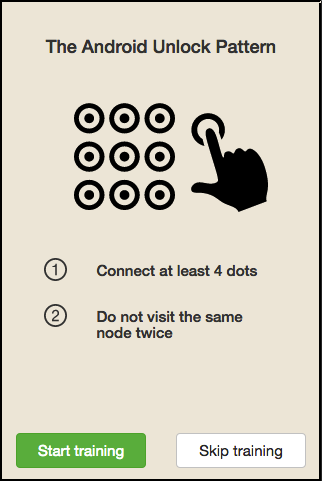
\includegraphics[scale=0.34]{pics/survey/rules}
          \label{fig:ALPintroduction}
        }
        \subfigure[Training mode]{
          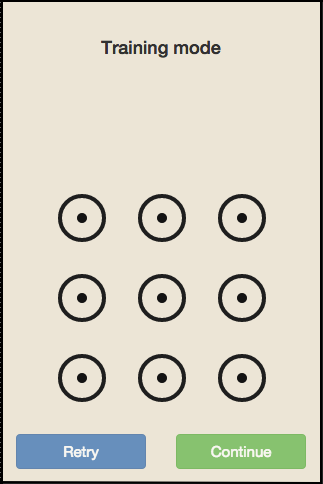
\includegraphics[scale=0.34]{pics/survey/training}
          \label{fig:trainingmode}
        }
        \caption{Survey screens}
        \label{fig:introductionviews}
      \end{figure}

    \subsection{Pattern Creation Process}
    After introducing the research and the Android Pattern Lock,  it is time to start collecting the three main selected patterns types; shopping account, smartphone, and banking account. The reason for dividing the pattern collection process into three separate patterns is to put the pattern creation into a context. The decision to add three patterns also works as a preventive measure for avoiding data being submitted by respondents just trying to finish the survey as fast as possible. 

    By introducing three separate pattern types instead of only one type, can introduce both positive and negative effects. When asking respondents to create a pattern for other types than its intended environment, some people might be confused. The choice of asking people to create a pattern for a banking account can for someone be an uncomfortable situation, might causing respondents to leave the survey. By asking the participants to create three patterns instead of one pattern takes more time and requires more attention and creativity from the participant. When asking respondents to create three patterns can introduce a situation where some respondents are creating the same pattern for all pattern types. 

    In the survey, respondents are asked to create a pattern for a shopping account, a smartphone, and a banking account. The three types are being carefully selected of how people would categorize different situations from a security point of view. As mentioned, the three pattern types are introduced to set the pattern creation process into context, avoiding dishonest attempts for answering the survey. 

    When collecting the patterns, it is desirable to copy the pattern creation process used by Android. The process consists of two steps: create a pattern of at least four connected dots, after that retype the same pattern for completing the process. Figure \ref{fig:androidpatterncreationprocess} shows the pattern creation process from a real Android smartphone. First, the user selects a pattern of at least four connected dots as illustrated in Figure \ref{fig:drawpattern}. Second, after creating a pattern, the user are asked to retype the same pattern as illustrated in Figure \ref{fig:confirmnewpattern}. If the redrawn pattern was correctly typed, the pattern creation process are finished. The pattern creation process used in the survey are visualized in Figure \ref{fig:patterncreationworkflow} and \ref{fig:createandretypepatterns}.

    \begin{figure}[H]
      \centering
      \subfigure[Draw pattern]{
        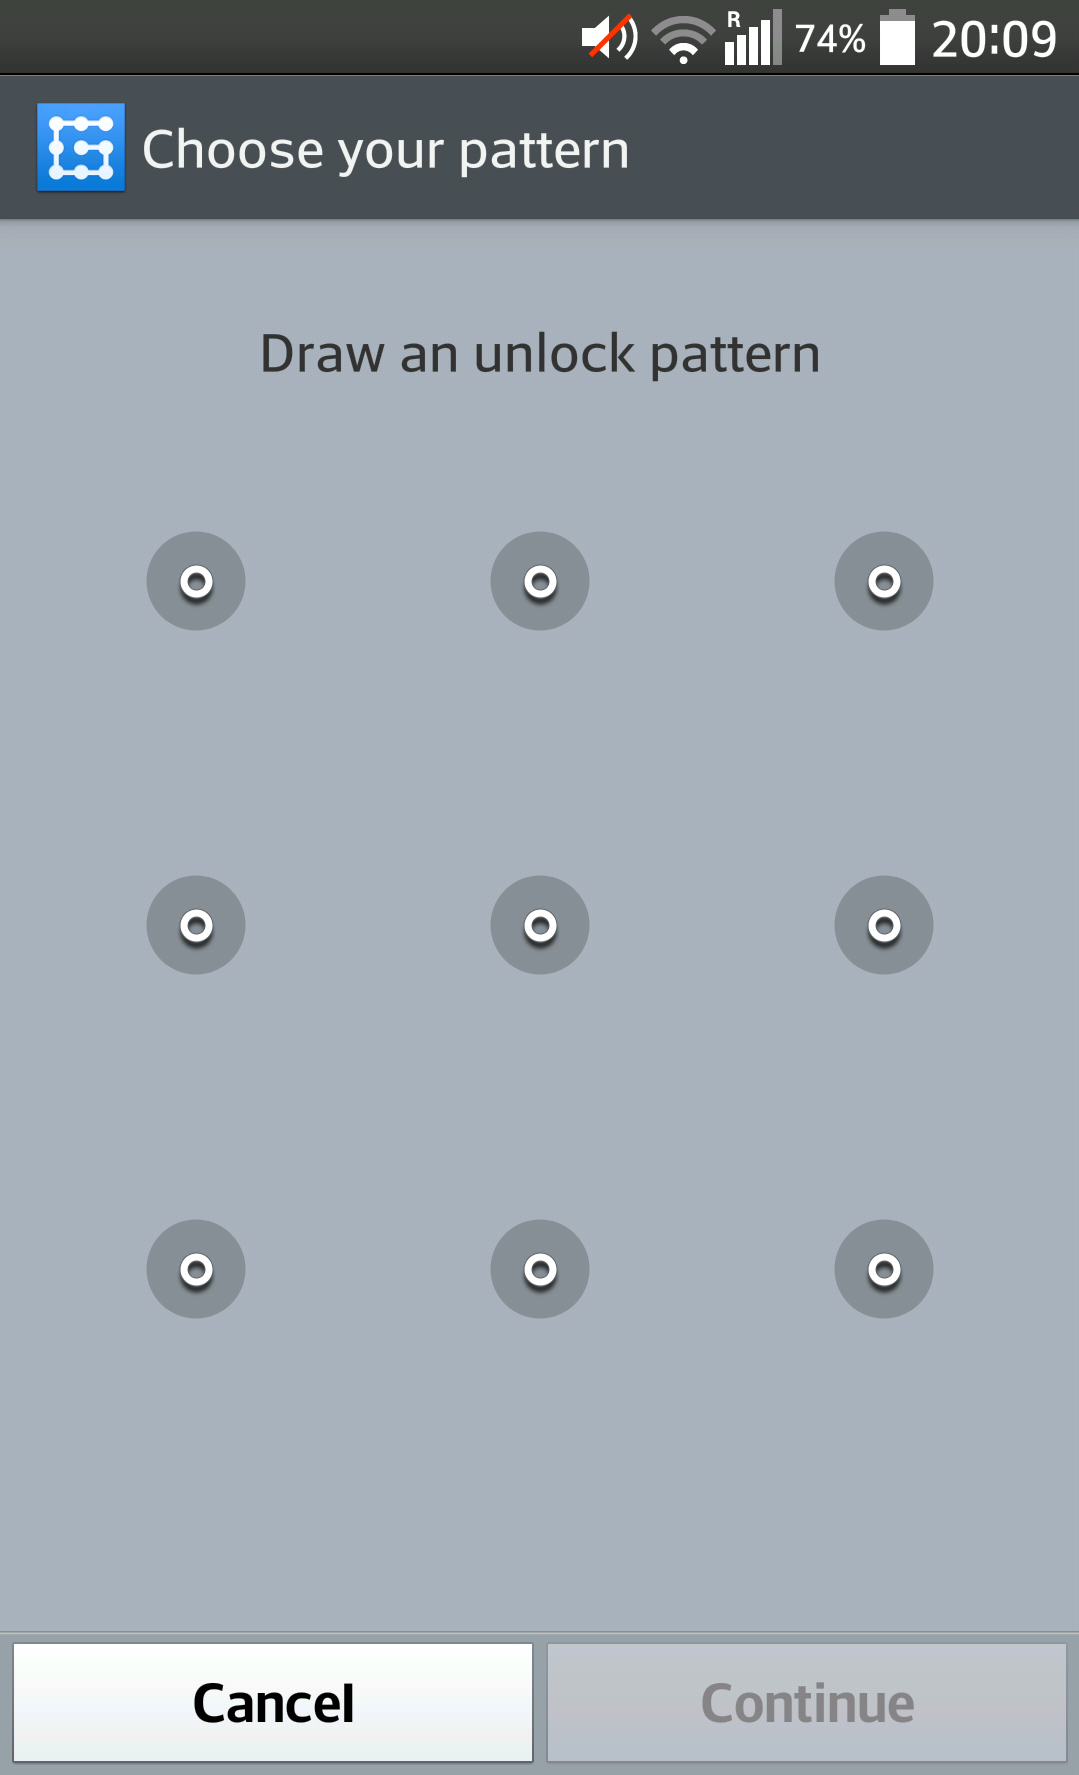
\includegraphics[scale=0.08]{pics/experiment/patternprocess3.png}
        \label{fig:drawpattern}
      }
      \subfigure[Pattern recorded]{
        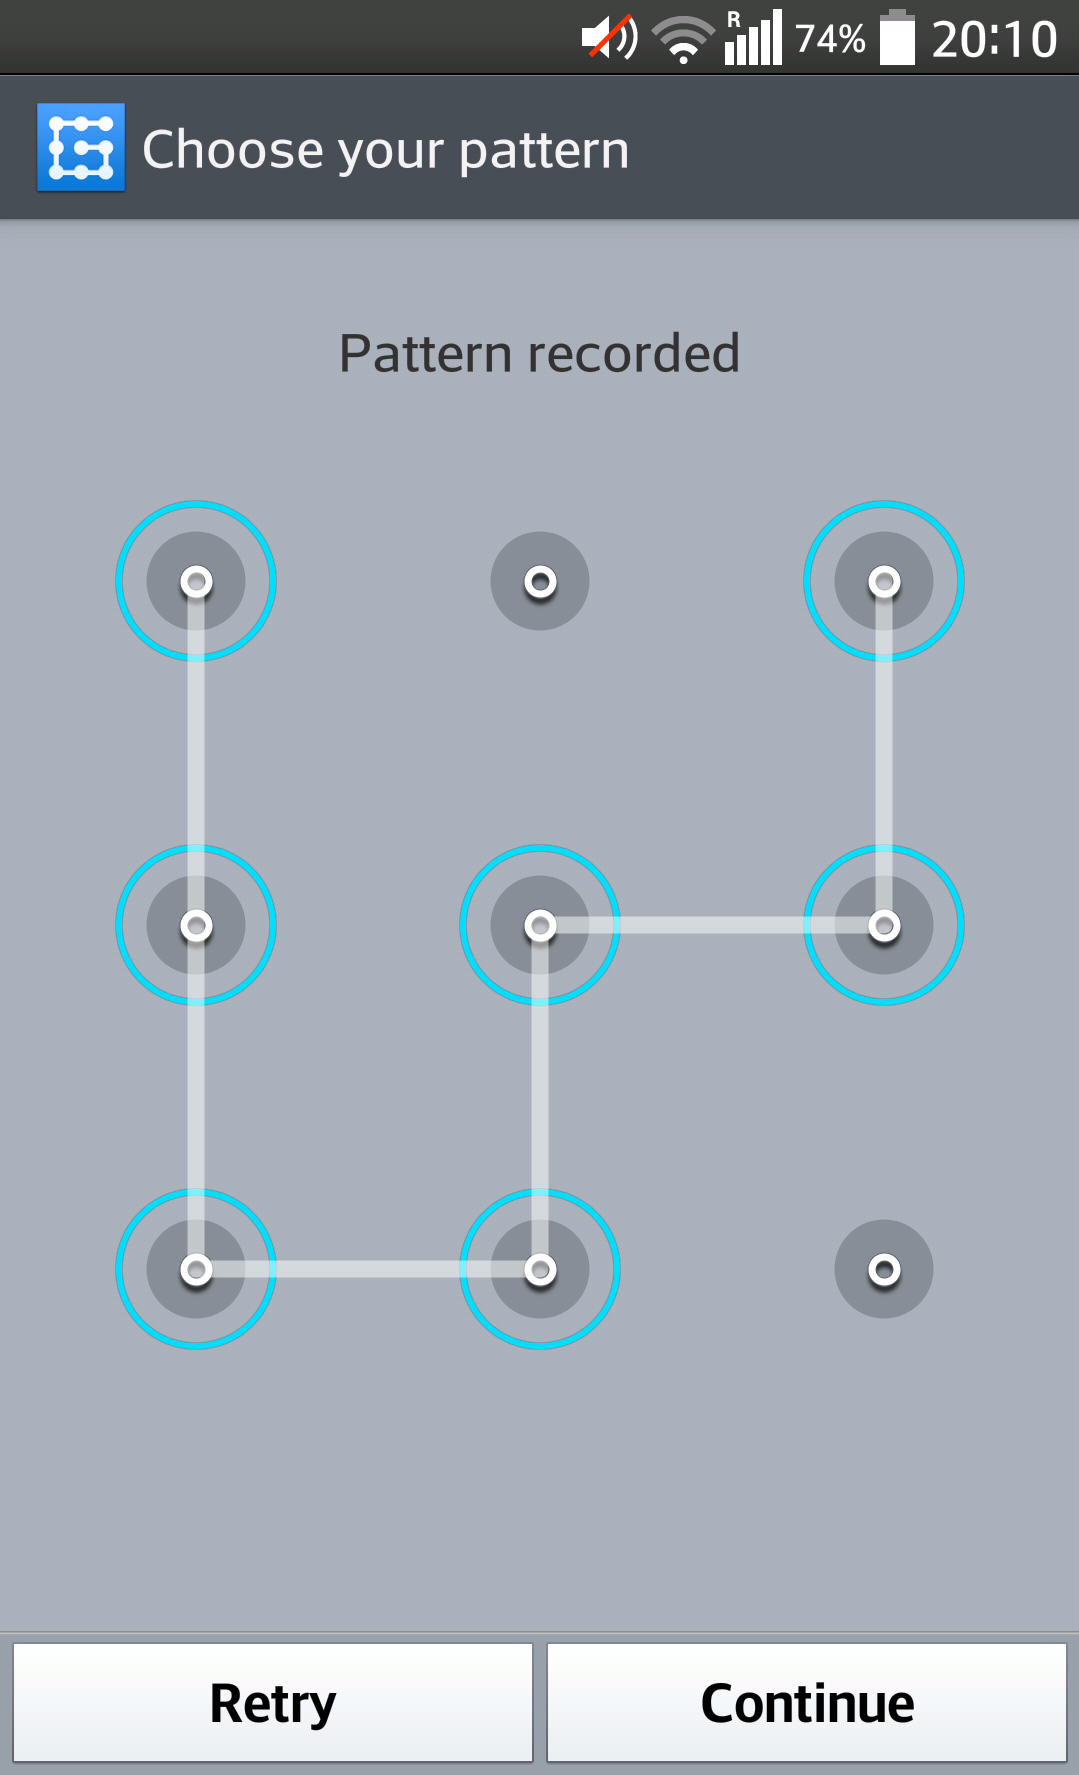
\includegraphics[scale=0.08]{pics/experiment/patternprocess4.png}
        \label{fig:patternrecorded}
      }\\
      \subfigure[Redraw pattern]{
        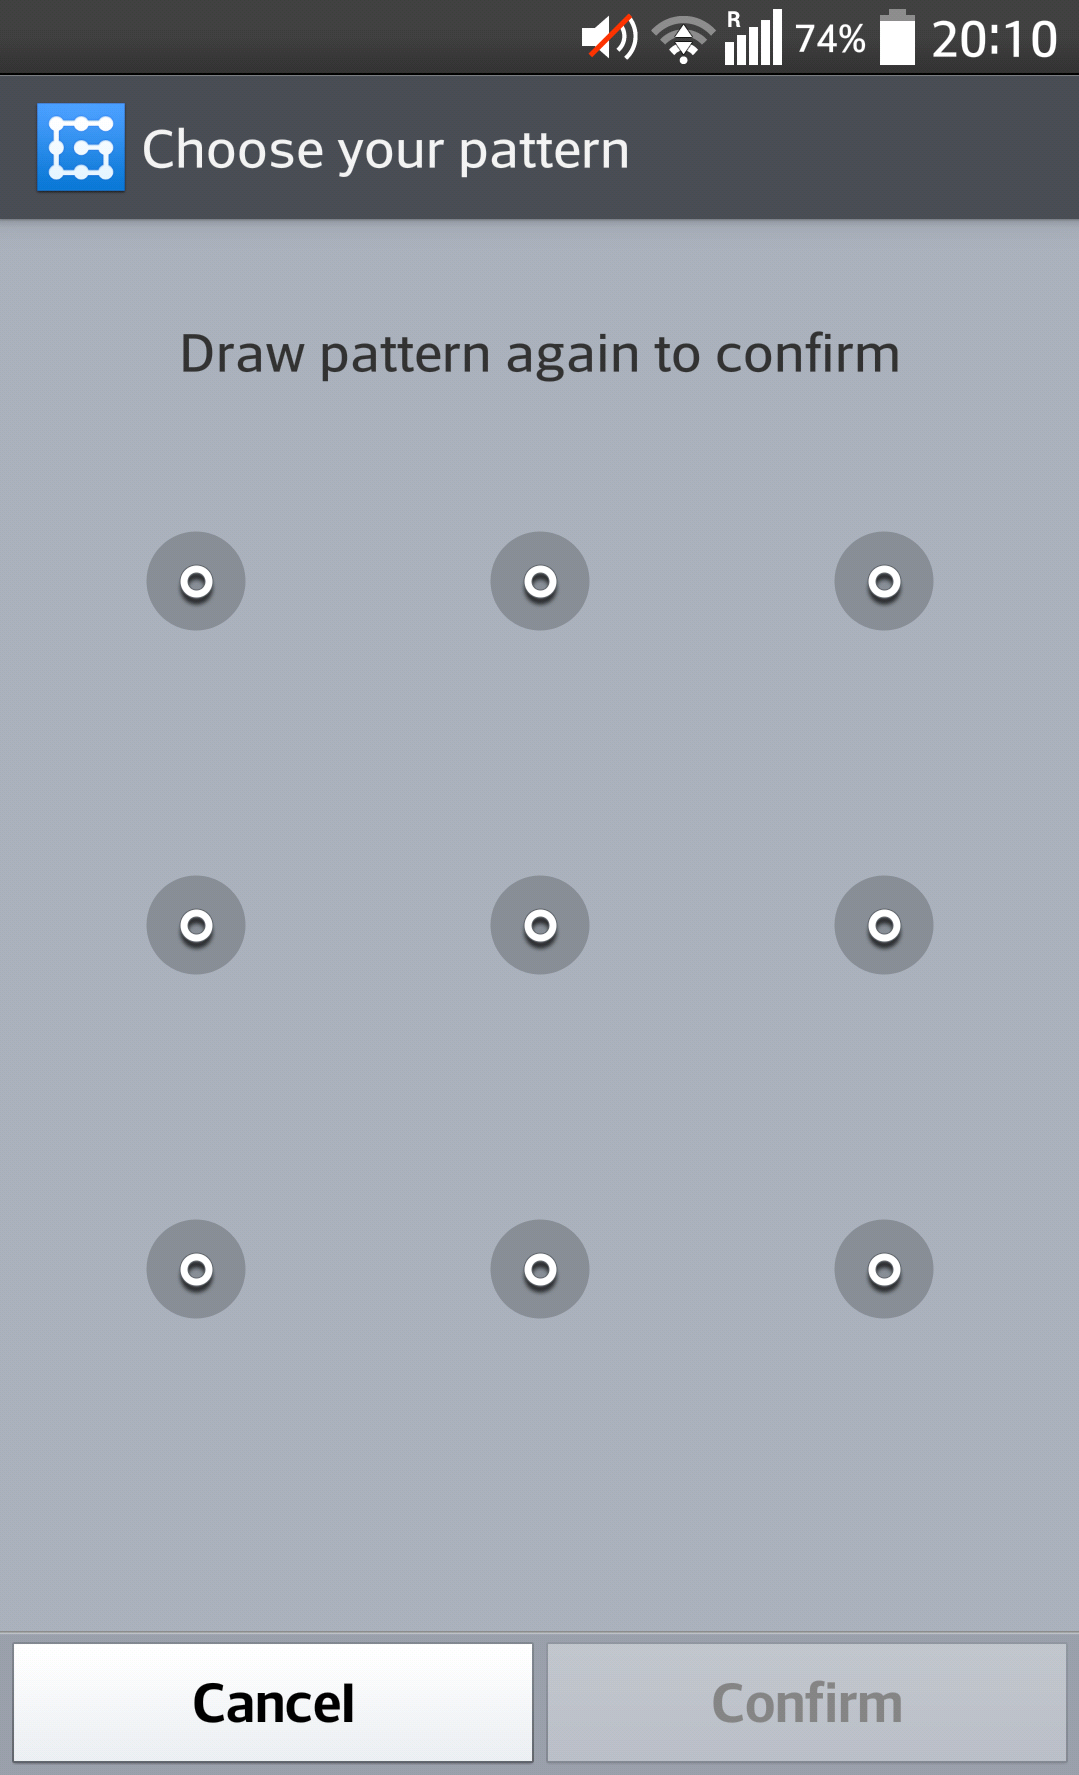
\includegraphics[scale=0.08]{pics/experiment/patternprocess5.png}
        \label{fig:redrawpattern}
      }
      \subfigure[Confirm new pattern]{
        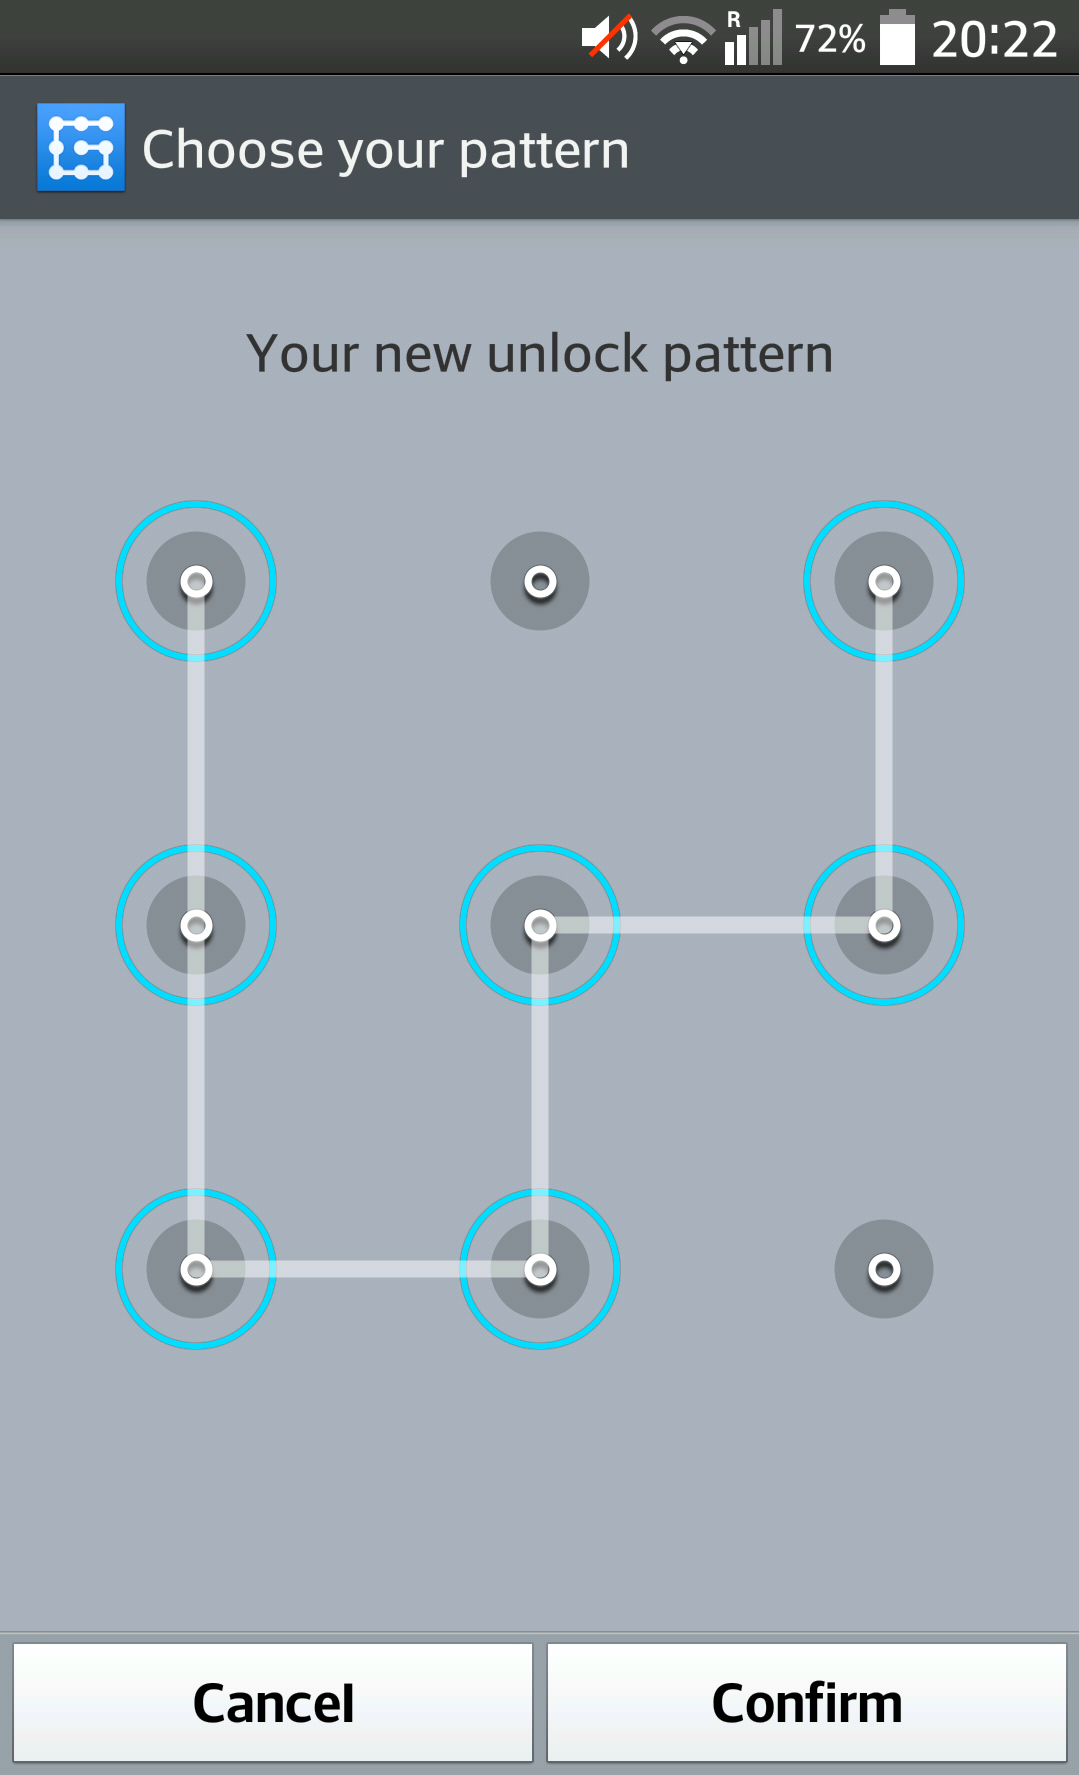
\includegraphics[scale=0.08]{pics/experiment/patternprocess1.png}
        \label{fig:confirmnewpattern}
      }
      \caption{The Android pattern creation process}
      \label{fig:androidpatterncreationprocess}
    \end{figure}

    \clearpage

    \begin{figure}[H]
      \centering
      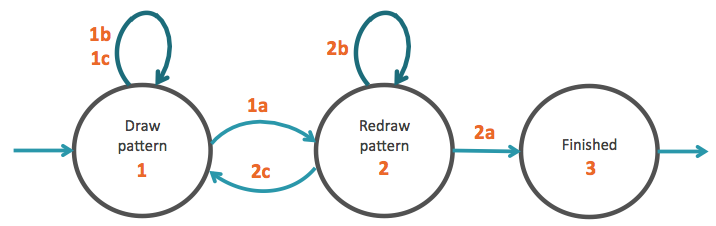
\includegraphics[width=\textwidth]{pics/experiment/patterncreationflow.png}
      \caption{Pattern creation workflow}
      \label{fig:patterncreationworkflow}
    \end{figure}

      \begin{enumerate}[leftmargin=0.3in]
        \item The first step is tp draw the pattern. The patter are drawn by connecting the nodes on the grid creating lines between the nodes (Figure \ref{fig:bankpattern}). The user will not be able to proceed before a valid pattern is drawn.
          \begin{enumerate}
            \item If the pattern is a valid pattern, the pattern turns green, and the message "pattern recorded" are shown. After, the user are able to press the {\it "Continue"} button to proceed to step 2 (Figure \ref{fig:validpatternrecorded}). 
            \item IIf the pattern not being valid pattern, the pattern turns red, and the message {\it "Connect at least 4 dots"} are shown (Figure \ref{fig:patternlengthtooshort}). The user can press the button {\it "Retry"}  for redrawing a new pattern.
            \item If a pattern drawn is a valid pattern, but the user want to create a different pattern, the user can always press the "Retry" button to reset the pattern already created. 
          \end{enumerate}
        \item When the respondent has created a valid pattern in step 1, they are proceeded to step 2 for redrawing the created pattern. The view is very similar to the view in step 1 beside the buttons and the text (Figure \ref{fig:retypepattern}).
          \begin{enumerate}
            \item If the user successfully redraws the pattern from step 1, the pattern turns green, and the message {\it "Correct!"} appears as in Figure \ref{fig:retypecorrect}. The user can complete the pattern creation process by clicking the green button {\it "Continue"} to proceed to step 3 and complete the pattern creation process.
            \item If the user unsuccessfully manages to redraw the pattern cerated in step 1, the pattern turns red, and the message "Not the same pattern" appears (Figure \ref{fig:retypewrong}). The user can try to remember the pattern and try to draw again. A situation like this can appear when the user do not remember the pattern or incorrectly draws the pattern.    
            \item If the user do not remember the pattern created at all, the {\it "Back"} button can be hit to go back to step 1 where the user are able to recreate a new pattern.  
          \end{enumerate}
        \item When the user successfully redraws the pattern in step 2, the pattern is successfully created.
      \end{enumerate}

    \begin{figure}[H]
      \centering
      \subfigure[Introduction to patterns]{
        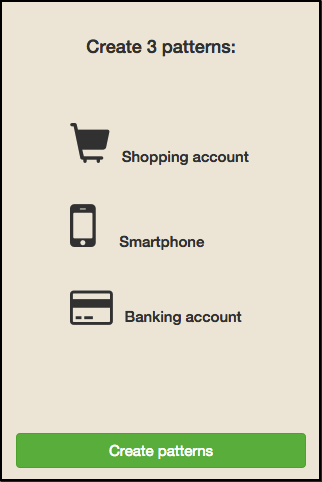
\includegraphics[scale=0.3]{pics/survey/pattern-introduction}
        \label{fig:introductiontopatterns}
      }
      \subfigure[Shopping pattern]{
        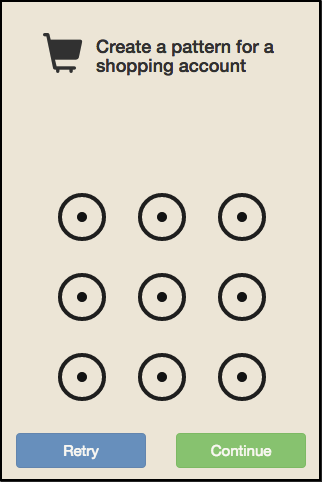
\includegraphics[scale=0.3]{pics/survey/shopping}
        \label{fig:shoppingpattern}
      }
      \subfigure[Smartphone pattern]{
        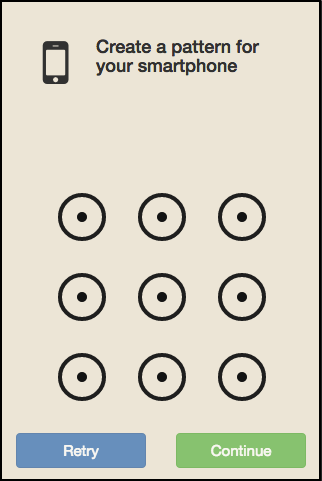
\includegraphics[scale=0.3]{pics/survey/smartphone}
        \label{fig:smartphonepattern}
      }
      \subfigure[Bank pattern]{
        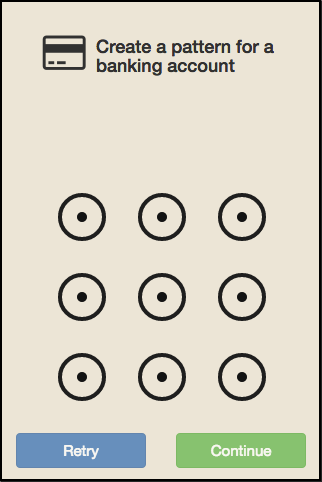
\includegraphics[scale=0.3]{pics/survey/bank}
        \label{fig:bankpattern}
      }
      \subfigure[Pattern length too short]{
        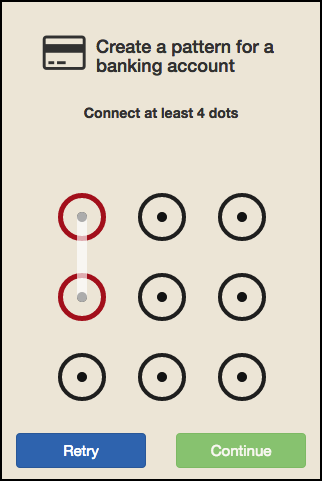
\includegraphics[scale=0.3]{pics/survey/not-valid-pattern-bank}
        \label{fig:patternlengthtooshort}
      }
      \subfigure[Valid pattern recorded]{
        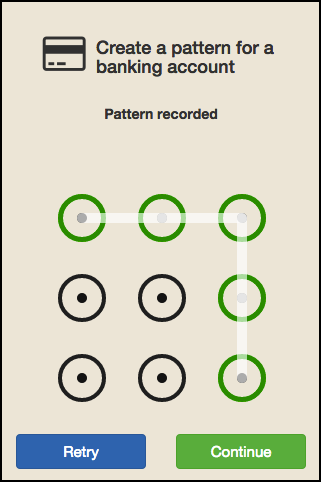
\includegraphics[scale=0.3]{pics/survey/pattern-recorded-bank}
        \label{fig:validpatternrecorded}
      }
      \subfigure[Retype pattern]{
        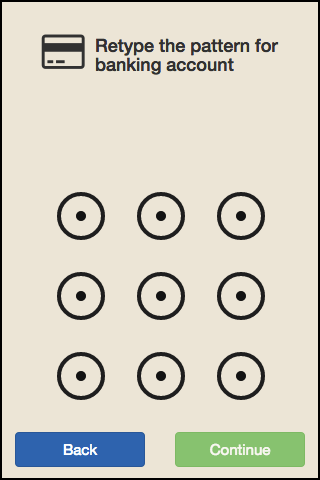
\includegraphics[scale=0.3]{pics/survey/retype-bank}
        \label{fig:retypepattern}
      }
      \subfigure[Retype wrong]{
        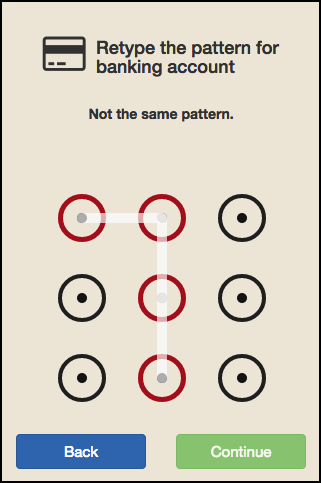
\includegraphics[scale=0.3]{pics/survey/not-valid-retype-bank}@
        \label{fig:retypewrong}
      }
      \subfigure[Retype correct]{
        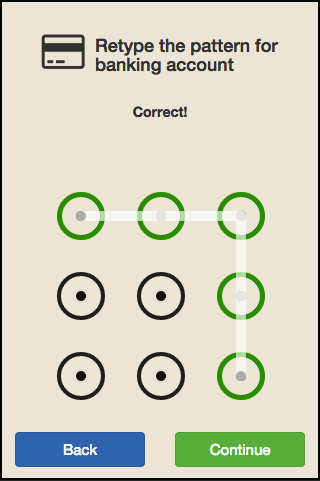
\includegraphics[scale=0.3]{pics/survey/retype-correct-bank}
        \label{fig:retypecorrect}
      }
      \caption{Survey - Create and retye patterns}
      \label{fig:createandretypepatterns}
    \end{figure}

  \clearpage 

  \subsection{Background information}
    After going through the pattern creation process for the three pattern types, the respondent will now be asked several questions about their mobile and personal characteristics. Figure \ref{fig:surveyquestoins} shows screenshots from the survey application and the questions asked. The views in Figure \ref{fig:surveyquestoins} is the final design used used for collecting data. The changes made during the design and implementation are described in Section \ref{sec:usabilitytestingsurvey}. 

    There are some core functionality implemented in these questions that is important to notice. {\it First}, the traditional list of alternatives are replaced by icons. As discussed in Section \ref{sec:requirementstosurvey}, it is important to customize the interface for easy interaction on a mobile touchscreen. The images used are easy to interact with because of its size, and it requires less text because of the semantic meaning of the icons used. The icons used in the survey has been tested in a own usability test that are described later in Section \ref{sec:usabilityicontest}. {\it Second}, to keep the user motivated, a progress bar is added to the views. The questions are listed after their appearance in the survey. Not all the questions are visualized in figure \ref{fig:surveyquestoins}, but all will be described in in detail in this section. 

    The first questions to be asked is the handsize of the respondent, ranged from small to extra large as visualized in Figure \ref{fig:handsizeview}. The question is a subjective categorization, and there is no way of doing any countermeasures for avoiding wrong classification. There is often a difference in hand size of genders, so the question is asking the respondents to categorize the size of their hand according to their gender. By specifically asking for hand size based on gender will give a more precise answer. The male respondents claiming to have a small hand will probably have a bigger hand compared to female respondents claiming to have a the same size. 

    Figure \ref{fig:handednessview} and \ref{fig:screensizeview} are the handedness of the respondent and the size of the screen used, respectively. Whether a person should be straight forward, where your dominant are either left- or right-hand. Screen size has the same problem as asking for the hand size, because how a respondent categorizes the screen size depends on the subjective evaluation made by the respondent. A countermeasure for having the possibility to evaluate respondents categorization of the screen sizes is to store the size of the screen in pixels. The task of storing the pixel width and height of the screen are stored automatically when the respondent selects the screen size.

    Figure \ref{fig:fingerusedview} and \ref{fig:handusedview} is questions asking for the hand and finger used for creating the patterns. Typically, a respondent will either use their left or right hand for holding the smartphone while interacting with the screen by using either the forefinger or the thumb. The option of using another finger than forefinger and thumb are also applied. Instead of using words like thumb and forefinger, a circle is applied to a hand indicating the finger used. 

    Figure \ref{fig:readingandwritingview} are asking about the reading and writing direction preferred by the respondent. The three alternatives includes a small example to avoid any misinterpretation of the icons. Figure \ref{fig:genderview}, \ref{fig:ageview}, and \ref{fig:experiencewithITSecurity} are asking about the respondent's gender, age, and experience with IT and security. The alternatives for gender are visualized by using a male and female icon. The last question asks whether the respondent have any experience with IT and security. The screens missing from Figure \ref{fig:surveyquestoins} are the question asking for the screenlock the respondent use, country, and the last screen thanking the respondents for participating. 
    

  \clearpage

    \begin{figure}[H]
      \centering
      \subfigure[Handsize]{
        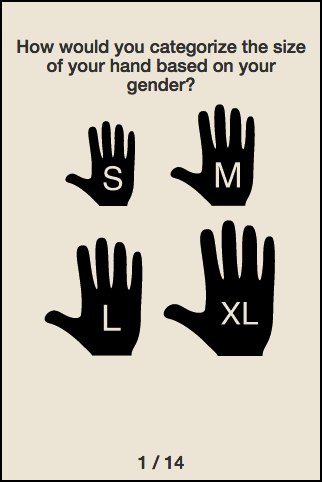
\includegraphics[scale=0.3]{pics/survey/handsize}
        \label{fig:handsizeview}
      }
      \subfigure[Handedness]{
        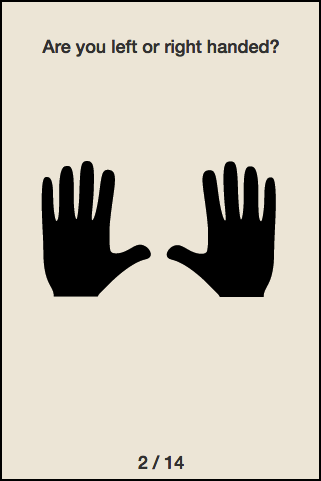
\includegraphics[scale=0.3]{pics/survey/handedness1}
        \label{fig:handednessview}
      }
      \subfigure[Screen size]{
        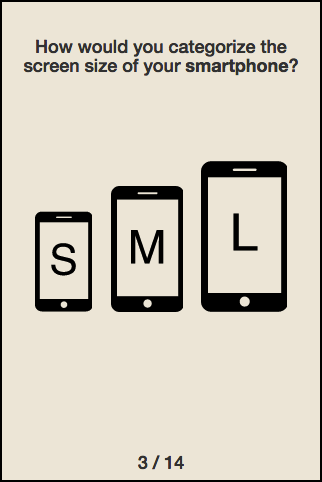
\includegraphics[scale=0.3]{pics/survey/screen}
        \label{fig:screensizeview}
      }
      \subfigure[Hand used when creating pattern]{
        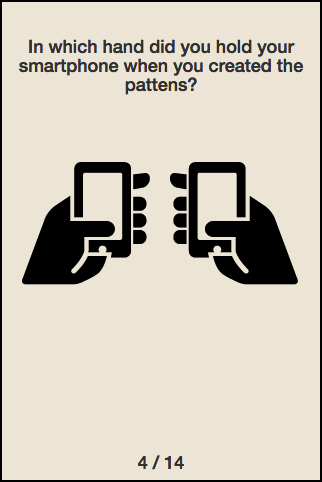
\includegraphics[scale=0.3]{pics/survey/handedness2}
        \label{fig:handusedview}
      }
      \subfigure[Finger used]{
        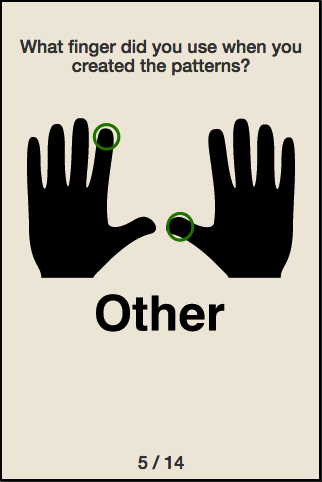
\includegraphics[scale=0.3]{pics/survey/finger}
        \label{fig:fingerusedview}
      }
      \subfigure[Reading/writing direction]{
        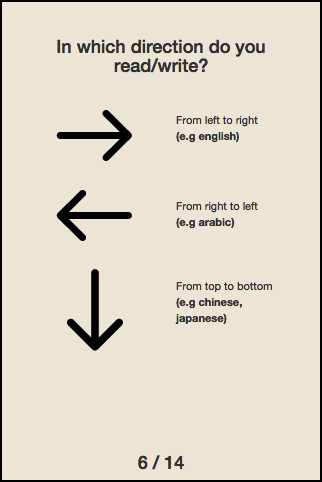
\includegraphics[scale=0.3]{pics/survey/reading}
        \label{fig:readingandwritingview}
      }
      \subfigure[Gender]{
        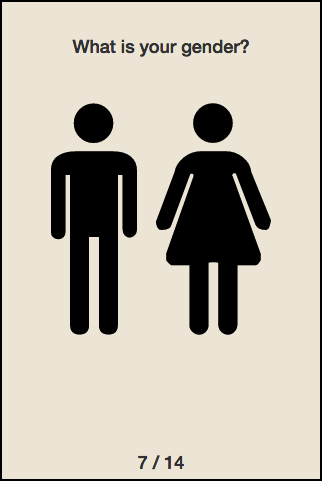
\includegraphics[scale=0.3]{pics/survey/gender}
        \label{fig:genderview}
      }
      \subfigure[Age]{
        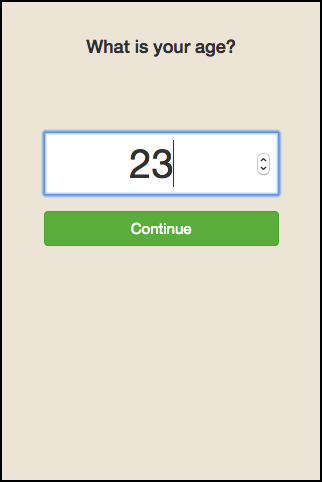
\includegraphics[scale=0.3]{pics/survey/age-2}
        \label{fig:ageview}
      }
      \subfigure[Experience]{
        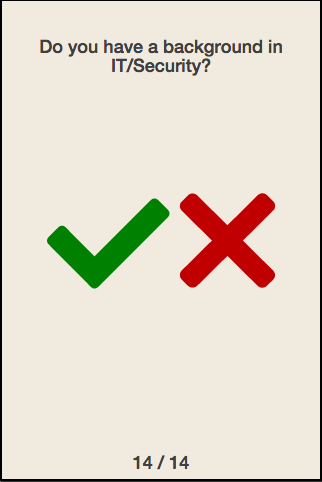
\includegraphics[scale=0.3]{pics/survey/experience2}
        \label{fig:experiencewithITSecurity}
      }
      \caption{Survey - Questions}
      \label{fig:surveyquestoins}
    \end{figure}

    \clearpage

    There is one special question in the survey that is not being mentioned until now; the mobile operating system used. This question is one of the hard questions to ask because it is no intuitive way for asking about the operating system of a mobile without using any technical terms. 

    Instead of listing all the possible mobile operating systems for mobile devices, the mobile operating system of the mobile is detected and visualized. In other words, the survey checks for the mobile OS and present what is being detected. With this information, a generic question like {\it "Is this your mobile operating system?"}, hence avoiding a long list asking {\it "Which one is your mobile OS?"}. The alternatives presented, \texttt{Yes}, \texttt{No}, and \texttt{Don't know}, are designed in way that the answer provided by the respondent are valuable whatever they select. For each mobile OS, each corresponding alternative are stored as \texttt{mobileOS\_yes}, \texttt{mobileOS\_no}, and \texttt{mobileOS\_unknown}.

    When the OS have been detected, one of the screens in Figure \ref{fig:mobileOSquestion} will show. It is implemented support for four different mobile operating systems that are covering the majority of the operating systems on smartphones: iOS, Android, Windows, and BlackBerry. Each OS will have the three alternatives yes, no, and question mark. 

    One pitfall is the formulation of the question. I should avoid any formulations stating that I detects their information. A question like {\it "It is detected that you have an Android phone. Is this correct?"} can be daunting, hence causing the respondents the feeling of being monitored. The feeling of someone knowing anything about you can be scary for anyone not knowing the technical details. The mobile operating system are easily detected on the client side with one line of code with {\it JavaScript}.

    \begin{figure}[H]
      \centering
      \subfigure[iOS]{
        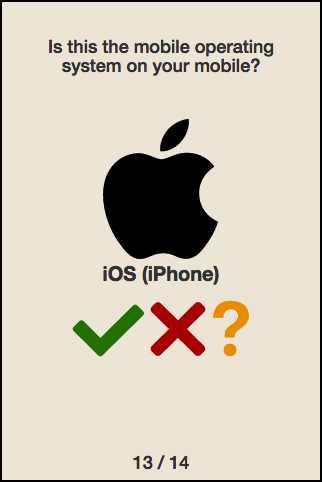
\includegraphics[scale=0.34]{pics/survey/ios}
      }
      \subfigure[Android]{
        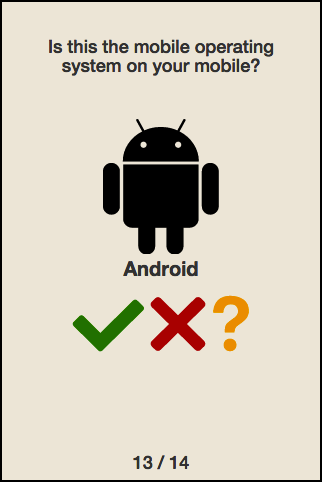
\includegraphics[scale=0.34]{pics/survey/android}
      }
      \subfigure[Windows]{
        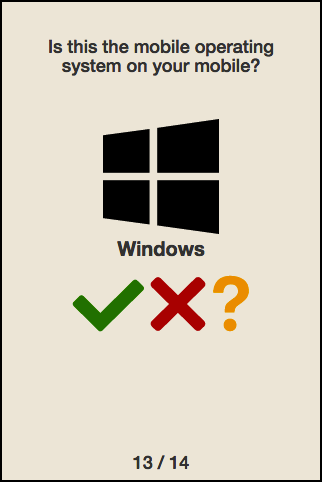
\includegraphics[scale=0.34]{pics/survey/windows}
      }
      \caption{Survey - Mobile OS}
      \label{fig:mobileOSquestion}
    \end{figure}
    \clearpage

    Figure \ref{fig:thefadingeffect} shows an example of what happens when the respondent clicks on an icon. When an icon is being press, the icons are highlighted by turning green like in Figure \ref{fig:selecticon}. When an icon is being clicked on, a slow fading effect starts for indicating the state changes to the next question. The fading effect are visualized in Figure \ref{fig:iconfadingout} and \ref{fig:iconfadedout}. When the question is faded out, the next question appears. The fading effect implemented is a cause of the described navigation requirements stated in Section \ref{sec:requirementstosurvey}. By using the automatic navigation while clicking on an image, the highlighting and the fading effect supports the respondent keeping track of the state. If a view is not utilizing icons, the fading effect is still used for indicating a change of state.

    \begin{figure}[H]
      \centering
      \subfigure[Select icon]{
        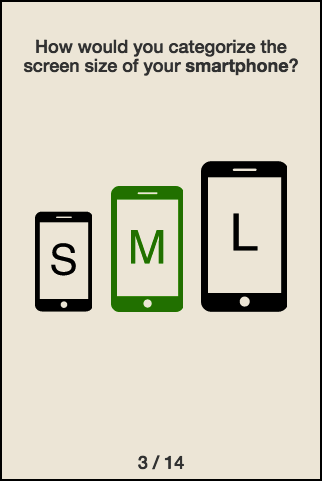
\includegraphics[scale=0.34]{pics/survey/icon-selected-1}
        \label{fig:selecticon}
      }
      \subfigure[Icon fading out]{
        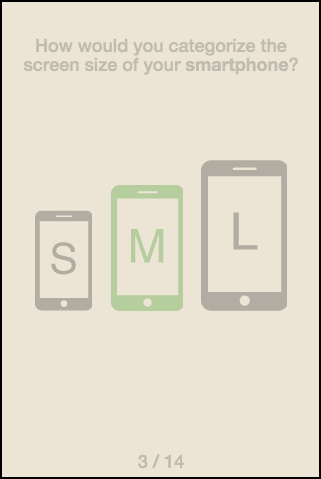
\includegraphics[scale=0.34]{pics/survey/icon-selected-3}
        \label{fig:iconfadingout}
      }
      \subfigure[Icon faded out]{
        
\includegraphics[scale=0.34]{pics/survey/icon-selected-4}
        \label{fig:iconfadedout}
      }
      \caption{Survey - Icon selecting effect}
      \label{fig:thefadingeffect}
    \end{figure}
